\chapter{Diseño e implementación de los modelos o técnicas necesarias}\label{ch: modelDesign}
En el capítulo \ref{ch: eda} se expuso la naturaleza espectral del problema, sería lógico pensar que una forma de reducir el ruido de una conversación sería filtrar para todas aquellas frecuencias que no sean la frecuencia fundamental y sus armónicos característicos del habla de una persona. Esta solución sería perfectamente válida y se ajusta a la necesidad del problema pero tiene un gran inconveniente, el tuneo fino y adaptable de los filtros.

Para poder filtrar las frecuencias fundamentales, éstas deben ser encontradas y esa no es tarea fácil. Además dichas frecuencias varían en el tiempo de modo que los filtros deben adaptarse a cada instante a la nuevas frecuencias, esto complica la tarea aún más. Existe una familia de filtros llamados \textit{comb}, peine, que consisten en una serie de picos equi-espaciados creando mediante retardos de la propia señal perfectamente válidos para la detección y filtrado de la frecuencia fundamental\cite{1035730}, de nuevo el tuneo fino es una tarea compleja. Por ello, este trabajo propone un sistema completo de redes neuronales en el cual no se aplican técnicas de clásicas de \gls{DSP}.

Dado que el en capítulo \ref{ch: eda} se presentaron los análisis en frecuencia y en tiempo, quedó de manifiesto que en el dominio de la frecuencia las pistas con ruido y sin él se diferencian mucho. Por esta razón el algoritmo que se propone en este trabajo se basa en el análisis de audio en el dominio de la frecuencia, para ello se deben pre-procesar los datos eligiendo unos parámetros que determinarán como serán los datos, a continuación se explican los algoritmos matemáticos de las transformaciones que se van a aplicar a las pistas de audio.

\section{Preprocesado de datos de audio para el modelo}
Los modelos se van a alimentar de \glspl{FFT} calculadas a partir de las muestras temporales de los audios. Estas \glspl{FFT} deben ser lo suficientemente precisas para poder reconstruir el audio pero sin usar una gran cantidad de muestras para no producir un retraso en la señal.

Se ha realizado una prueba experimental para calcular a que tasa de muestreo el audio sigue siendo posible reconstruir. A menor tasa de muestreo, para la misma resolución en frecuencia, la \gls{FFT} resultante tiene menos puntos, i.e., menor carga computacional. Es importante este ajuste porque reducir la tasa de muestreo a la mitad o un cuarto implica reducir el vector de entrada de la red a la mitad o un cuarto, respectivamente. Adicionalmente sólo son procesados la mitad de los datos de la salida de la transformada de Fourier. Esto es debido a que la respuesta de una transformada es un vector de números complejos y de éstos sólo se procesa el módulo. La fase se deja intacta y se usa para reconstruir el vector complejo junto con el módulo que sale del modelo. La figura \ref{fig: model_schema} presenta un esquema de cuáles son las entradas y salidas del modelo.

\begin{figure}[ht!]
	\centering
	\resizebox{\textwidth}{!}{
		\begin{tikzpicture}
		\tikzstyle{box} = [draw,inner sep=7,minimum size=57,line 
		width=1, very thick, draw=black, fill=black!20, text width=100, text centered]
		\tikzstyle{invisible} = [outer sep=0,inner sep=0,minimum size=0]
		\tikzstyle{stealth} = [-stealth, very thick]
		\begin{scope}[shift={(0.5,0)}]		
		\begin{scope}[shift={(-3.5,3.1)}, scale=0.5]
		\node [invisible] at (-1.2,1.7) {$FFT_n$};
		\draw (-3,0.5) node [invisible] {} -- (-2.8,0.3) node [invisible] {} -- (-2.6,0.2) node [invisible] {} -- (-2.4,0.8) node [invisible] {} -- (-2.2,0.2) node [invisible] {} -- (-2,0.3) node [invisible] {} -- (-1.9,0.2) node [invisible] {} -- (-1.8,0.4) node [invisible] {} -- (-1.7,0.2) node [invisible] {} -- (-1.6,1.4) node [invisible] {} -- (-1.5,0.2) node [invisible] {} -- (-1.3,0.3) node [invisible] (v4) {};
		\node [invisible] (v2) at (-3,1.6) {};
		\node [invisible] (v1) at (-3,-0.4) {};
		\node [invisible] (v3) at (0.6,-0.4) {};
		\draw [stealth] (v1) edge (v2);
		\draw [stealth] (v1) edge (v3);
		\draw [stealth](v4);
		\draw (v4) -- (-1.2,0.2) node [invisible] {} -- (-1.1,0.4) node [invisible] {} -- (-1,0.2) node [invisible] {} -- (-0.8,0.8) node [invisible] {} -- (-0.7,0.2) node [invisible] {} -- (-0.5,0.3) node [invisible] {} -- (-0.4,0.2) node [invisible] {} -- (-0.2,0.3) node [invisible] {} -- (-0.1,0.2) node [invisible] {} -- (0.1,1.1) node [invisible] {} -- (0.3,0.2) node [invisible] {};
		\end{scope}
		\begin{scope}[shift={(-3.1,1.8)}, scale=0.5]
		\node [invisible] at (-1.2,1.7) {$FFT_{n-1}$};
		\draw (-3,0.5) node [invisible] {} -- (-2.8,0.3) node [invisible] {} -- (-2.6,0.2) node [invisible] {} -- (-2.4,0.8) node [invisible] {} -- (-2.2,0.2) node [invisible] {} -- (-2,0.3) node [invisible] {} -- (-1.9,0.2) node [invisible] {} -- (-1.8,0.4) node [invisible] {} -- (-1.7,0.2) node [invisible] {} -- (-1.6,1.4) node [invisible] {} -- (-1.5,0.2) node [invisible] {} -- (-1.3,0.3) node [invisible] (v4) {};
		\node [invisible] (v2) at (-3,1.6) {};
		\node [invisible] (v1) at (-3,-0.4) {};
		\node [invisible] (v3) at (0.6,-0.4) {};
		\draw [stealth] (v1) edge (v2);
		\draw [stealth] (v1) edge (v3);
		\draw [stealth](v4);
		\draw (v4) -- (-1.2,0.2) node [invisible] {} -- (-1.1,0.4) node [invisible] {} -- (-1,0.2) node [invisible] {} -- (-0.8,0.8) node [invisible] {} -- (-0.7,0.2) node [invisible] {} -- (-0.5,0.3) node [invisible] {} -- (-0.4,0.2) node [invisible] {} -- (-0.2,0.3) node [invisible] {} -- (-0.1,0.2) node [invisible] {} -- (0.1,1.1) node [invisible] {} -- (0.3,0.2) node [invisible] {};
		\end{scope}
		\begin{scope}[shift={(-1.5,-0.9)}, scale=0.5]
		\node [invisible] at (-1.2,1.7) {$FFT_2$};
		\draw (-3,0.5) node [invisible] {} -- (-2.8,0.3) node [invisible] {} -- (-2.6,0.2) node [invisible] {} -- (-2.4,0.8) node [invisible] {} -- (-2.2,0.2) node [invisible] {} -- (-2,0.3) node [invisible] {} -- (-1.9,0.2) node [invisible] {} -- (-1.8,0.4) node [invisible] {} -- (-1.7,0.2) node [invisible] {} -- (-1.6,1.4) node [invisible] {} -- (-1.5,0.2) node [invisible] {} -- (-1.3,0.3) node [invisible] (v4) {};
		\node [invisible] (v2) at (-3,1.6) {};
		\node [invisible] (v1) at (-3,-0.4) {};
		\node [invisible] (v3) at (0.6,-0.4) {};
		\draw [stealth] (v1) edge (v2);
		\draw [stealth] (v1) edge (v3);
		\draw [stealth](v4);
		\draw (v4) -- (-1.2,0.2) node [invisible] {} -- (-1.1,0.4) node [invisible] {} -- (-1,0.2) node [invisible] {} -- (-0.8,0.8) node [invisible] {} -- (-0.7,0.2) node [invisible] {} -- (-0.5,0.3) node [invisible] {} -- (-0.4,0.2) node [invisible] {} -- (-0.2,0.3) node [invisible] {} -- (-0.1,0.2) node [invisible] {} -- (0.1,1.1) node [invisible] {} -- (0.3,0.2) node [invisible] {};
		\end{scope}
		\begin{scope}[shift={(-1.1,-2.2)}, scale=0.5]
		\node [invisible] at (-1.2,1.7) {$FFT_1$};
		\draw (-3,0.5) node [invisible] {} -- (-2.8,0.3) node [invisible] {} -- (-2.6,0.2) node [invisible] {} -- (-2.4,0.8) node [invisible] {} -- (-2.2,0.2) node [invisible] {} -- (-2,0.3) node [invisible] {} -- (-1.9,0.2) node [invisible] {} -- (-1.8,0.4) node [invisible] {} -- (-1.7,0.2) node [invisible] {} -- (-1.6,1.4) node [invisible] {} -- (-1.5,0.2) node [invisible] {} -- (-1.3,0.3) node [invisible] (v4) {};
		\node [invisible] (v2) at (-3,1.6) {};
		\node [invisible] (v1) at (-3,-0.4) {};
		\node [invisible] (v3) at (0.6,-0.4) {};
		\draw [stealth] (v1) edge (v2);
		\draw [stealth] (v1) edge (v3);
		\draw [stealth](v4);
		\draw (v4) -- (-1.2,0.2) node [invisible] {} -- (-1.1,0.4) node [invisible] {} -- (-1,0.2) node [invisible] {} -- (-0.8,0.8) node [invisible] {} -- (-0.7,0.2) node [invisible] {} -- (-0.5,0.3) node [invisible] {} -- (-0.4,0.2) node [invisible] {} -- (-0.2,0.3) node [invisible] {} -- (-0.1,0.2) node [invisible] {} -- (0.1,1.1) node [invisible] {} -- (0.3,0.2) node [invisible] {};
		\end{scope}
		\node [circle, fill] at (-3.6,1.2) {};
		\node [circle, fill] at (-3.2,0.8) {};
		\node [circle, fill] at (-2.8,0.4) {};
		\draw [dashed, thick] (-5.5,6) node [invisible] (v5) {} -- (-5.5,-3.5) -- (-0.5,-3.5) -- (-0.5,6) -- (v5);
		\node [invisible] (v6) at (-0.5,0.75) {};
		\end{scope}
		
		\begin{scope}[shift={(10.5,0)}]		
		\begin{scope}[shift={(-1.2,3.1)}, scale=0.5]
		\node [invisible] at (-1.2,1.7) {$FFT_n$};
		\draw (-3,0.5) node [invisible] {} -- (-2.8,0.3) node [invisible] {} -- (-2.6,0.2) node [invisible] {} -- (-2.4,0.8) node [invisible] {} -- (-2.2,0.2) node [invisible] {} -- (-2,0.3) node [invisible] {} -- (-1.9,0.2) node [invisible] {} -- (-1.8,0.4) node [invisible] {} -- (-1.7,0.2) node [invisible] {} -- (-1.6,1.4) node [invisible] {} -- (-1.5,0.2) node [invisible] {} -- (-1.3,0.3) node [invisible] (v4) {};
		\node [invisible] (v2) at (-3,1.6) {};
		\node [invisible] (v1) at (-3,-0.4) {};
		\node [invisible] (v3) at (0.6,-0.4) {};
		\draw [stealth] (v1) edge (v2);
		\draw [stealth] (v1) edge (v3);
		\draw [stealth](v4);
		\draw (v4) -- (-1.2,0.2) node [invisible] {} -- (-1.1,0.4) node [invisible] {} -- (-1,0.2) node [invisible] {} -- (-0.8,0.8) node [invisible] {} -- (-0.7,0.2) node [invisible] {} -- (-0.5,0.3) node [invisible] {} -- (-0.4,0.2) node [invisible] {} -- (-0.2,0.3) node [invisible] {} -- (-0.1,0.2) node [invisible] {} -- (0.1,1.1) node [invisible] {} -- (0.3,0.2) node [invisible] {};
		\end{scope}
		\begin{scope}[shift={(-1.7,1.8)}, scale=0.5]
		\node [invisible] at (-1.2,1.7) {$FFT_{n-1}$};
		\draw (-3,0.5) node [invisible] {} -- (-2.8,0.3) node [invisible] {} -- (-2.6,0.2) node [invisible] {} -- (-2.4,0.8) node [invisible] {} -- (-2.2,0.2) node [invisible] {} -- (-2,0.3) node [invisible] {} -- (-1.9,0.2) node [invisible] {} -- (-1.8,0.4) node [invisible] {} -- (-1.7,0.2) node [invisible] {} -- (-1.6,1.4) node [invisible] {} -- (-1.5,0.2) node [invisible] {} -- (-1.3,0.3) node [invisible] (v4) {};
		\node [invisible] (v2) at (-3,1.6) {};
		\node [invisible] (v1) at (-3,-0.4) {};
		\node [invisible] (v3) at (0.6,-0.4) {};
		\draw [stealth] (v1) edge (v2);
		\draw [stealth] (v1) edge (v3);
		\draw [stealth](v4);
		\draw (v4) -- (-1.2,0.2) node [invisible] {} -- (-1.1,0.4) node [invisible] {} -- (-1,0.2) node [invisible] {} -- (-0.8,0.8) node [invisible] {} -- (-0.7,0.2) node [invisible] {} -- (-0.5,0.3) node [invisible] {} -- (-0.4,0.2) node [invisible] {} -- (-0.2,0.3) node [invisible] {} -- (-0.1,0.2) node [invisible] {} -- (0.1,1.1) node [invisible] {} -- (0.3,0.2) node [invisible] {};
		\end{scope}
		\begin{scope}[shift={(-3.2,-0.9)}, scale=0.5]
		\node [invisible] at (-1.2,1.7) {$FFT_2$};
		\draw (-3,0.5) node [invisible] {} -- (-2.8,0.3) node [invisible] {} -- (-2.6,0.2) node [invisible] {} -- (-2.4,0.8) node [invisible] {} -- (-2.2,0.2) node [invisible] {} -- (-2,0.3) node [invisible] {} -- (-1.9,0.2) node [invisible] {} -- (-1.8,0.4) node [invisible] {} -- (-1.7,0.2) node [invisible] {} -- (-1.6,1.4) node [invisible] {} -- (-1.5,0.2) node [invisible] {} -- (-1.3,0.3) node [invisible] (v4) {};
		\node [invisible] (v2) at (-3,1.6) {};
		\node [invisible] (v1) at (-3,-0.4) {};
		\node [invisible] (v3) at (0.6,-0.4) {};
		\draw [stealth] (v1) edge (v2);
		\draw [stealth] (v1) edge (v3);
		\draw [stealth](v4);
		\draw (v4) -- (-1.2,0.2) node [invisible] {} -- (-1.1,0.4) node [invisible] {} -- (-1,0.2) node [invisible] {} -- (-0.8,0.8) node [invisible] {} -- (-0.7,0.2) node [invisible] {} -- (-0.5,0.3) node [invisible] {} -- (-0.4,0.2) node [invisible] {} -- (-0.2,0.3) node [invisible] {} -- (-0.1,0.2) node [invisible] {} -- (0.1,1.1) node [invisible] {} -- (0.3,0.2) node [invisible] {};
		\end{scope}
		\begin{scope}[shift={(-3.7,-2.2)}, scale=0.5]
		\node [invisible] at (-1.2,1.7) {$FFT_1$};
		\draw (-3,0.5) node [invisible] {} -- (-2.8,0.3) node [invisible] {} -- (-2.6,0.2) node [invisible] {} -- (-2.4,0.8) node [invisible] {} -- (-2.2,0.2) node [invisible] {} -- (-2,0.3) node [invisible] {} -- (-1.9,0.2) node [invisible] {} -- (-1.8,0.4) node [invisible] {} -- (-1.7,0.2) node [invisible] {} -- (-1.6,1.4) node [invisible] {} -- (-1.5,0.2) node [invisible] {} -- (-1.3,0.3) node [invisible] (v4) {};
		\node [invisible] (v2) at (-3,1.6) {};
		\node [invisible] (v1) at (-3,-0.4) {};
		\node [invisible] (v3) at (0.6,-0.4) {};
		\draw [stealth] (v1) edge (v2);
		\draw [stealth] (v1) edge (v3);
		\draw [stealth](v4);
		\draw (v4) -- (-1.2,0.2) node [invisible] {} -- (-1.1,0.4) node [invisible] {} -- (-1,0.2) node [invisible] {} -- (-0.8,0.8) node [invisible] {} -- (-0.7,0.2) node [invisible] {} -- (-0.5,0.3) node [invisible] {} -- (-0.4,0.2) node [invisible] {} -- (-0.2,0.3) node [invisible] {} -- (-0.1,0.2) node [invisible] {} -- (0.1,1.1) node [invisible] {} -- (0.3,0.2) node [invisible] {};
		\end{scope}
		\node [circle, fill] at (-2.8,1.2) {};
		\node [circle, fill] at (-3.2,0.8) {};
		\node [circle, fill] at (-3.6,0.4) {};
		\draw [dashed, thick] (-5.5,6) node [invisible] (v5) {} -- (-5.5,-3.5) -- (-0.5,-3.5) -- (-0.5,6) -- (v5);
		\node [invisible] (v8) at (-5.5,0.75) {};
		\end{scope}
		
		\node [box,text width=60] (v7) at (2.5,0.75) {Modelo};
		
		
		\node [invisible] at (-2.5,5.5) {Módulo de FFT con ruido};
		\node [invisible] at (7.5,5.5) {Módulo de FFT sin ruido};
		\draw [stealth] (v6) edge (v7);
		\draw [stealth] (v7) edge (v8);
		\node [box] (v9) at (-8.5,7) {$Tiempo\xrightarrow{FFT}Frecuencia$};
		\node [box] (v10) at (13.5,7) {$Frecuencia\xrightarrow{iFFT}Tiempo$};
		\node [invisible] (v11) at (-5,0.75) {};
		\node [invisible] (v12) at (10,0.75) {};
		\draw [stealth,out=0,in=180] (v9) edge node[anchor=south]{Fase} (v10);
		\draw [stealth,out=0,in=180] (v9) edge node[anchor=east]{Módulo}(v11);
		\draw [stealth,out=0,in=180] (v12) edge node[anchor=west]{Módulo}(v10);
		\end{tikzpicture}
	}      
	\caption{Esquema de las entradas y salidas de datos del modelo}
	\label{fig: model_schema}
\end{figure}

Dado que el tamaño de la transformada y la precisión en frecuencia depende de la tasa de muestreo de la señal, el algoritmo debe funcionar a tasa de muestreo fija. Es decir, sea cual fuere la tasa de muestreo en generación de datos, éstos deben ser re-muestreados, en inglés \textit{resampling}, a la tasa de muestreo objetivo, previo al cálculo de la transformada. Igualmente, el número de puntos de la transformada debe ser fijo. La cadena completa de procesado de señal se muestra en \ref{fig: model_chain}.
 
\begin{figure}[ht!]
	\centering
	\resizebox{1.1\textwidth}{!}{
		\begin{tikzpicture}
		\tikzstyle{box} = [draw,inner sep=7,minimum size=57,line 
		width=1, very thick, draw=black, fill=black!20, text width=80, text centered]
		\tikzstyle{invisible} = [outer sep=0,inner sep=0,minimum size=0]
		\tikzstyle{stealth} = [-stealth, very thick]
		\begin{scope} [scale=0.1, shift={(-112.5,10)}]
		\draw [very thick] (-2,0.5) arc (0:-180:1.5);
		\draw [very thick] (-2,3.5) arc (0:180:1.5);
		\node [invisible] (v1) at (-5,3.5) {};
		\node [invisible] (v3) at (-2,3.5) {};
		\node [invisible] (v2) at (-5,0.5) {};
		\node [invisible] (v4) at (-2,0.5) {};
		\draw [very thick] (v1) edge (v2);
		\draw [very thick] (v3) edge (v4);
		\node [invisible] (v9) at (-5,3) {};
		\node [invisible] (v10) at (-4,3) {};
		\node [invisible] (v11) at (-5,2) {};
		\node [invisible] (v12) at (-4,2) {};
		\node [invisible] (v13) at (-5,1) {};
		\node [invisible] (v14) at (-4,1) {};
		\node [invisible] (v15) at (-2,1) {};
		\node [invisible] (v16) at (-3,1) {};
		\node [invisible] (v17) at (-2,2) {};
		\node [invisible] (v18) at (-3,2) {};
		\node [invisible] (v19) at (-2,3) {};
		\node [invisible] (v20) at (-3,3) {};
		\draw [very thick] (-1.5,0.5) arc (0:-180:2);
		\node [invisible] (v7) at (-3.5,-1.5) {};
		\node [invisible] (v8) at (-3.5,-2.5) {};
		\node [invisible] (v5) at (-5.5,-2.5) {};
		\node [invisible] (v6) at (-1.5,-2.5) {};
		\draw [very thick] (v5) edge (v6);
		\draw [very thick] (v7) edge (v8);
		\draw [very thick] (v9) edge (v10);
		\draw [very thick] (v11) edge (v12);
		\draw [very thick] (v13) edge (v14);
		\draw [very thick] (v15) edge (v16);
		\draw [very thick] (v17) edge (v18);
		\draw [very thick] (v19) edge (v20);
		\end{scope}
		\node [box] (v23) at (-3,1) {Adaptación de la tasa de muestreo a $11025 \frac{muestras}{segundo}$};
		\node [box] (v22) at (-8.1,1) {Analógico $\xrightarrow{}$ Digital};
		\node [invisible] (v21) at (-11,1) {};
		\node [box] (v24) at (2.5,1) {FFT de $1024~muestras$};
		\node [box, minimum size=40] (v30) at (8.5,2.5) {Módulo};
		\node [box, minimum size=40] (v31) at (8.5,-0.5) {Fase};
		\node [box] (v26) at (2.5,-4.5) {$mod\cdot e^{j\cdot fase}$};
		\node [box] (v27) at (-3,-4.5) {iFFT};
		\node [box] (v28) at (-8.1,-4.5) {Analógico $\xleftarrow{}$ Digital};
		\begin{scope}[scale=0.4, shift={(-35.6,-8.15)}, xscale=-1]
		\draw [rounded corners, very thick, fill] (-7,-2.6) node [invisible] (v25) {} -- (-7,-3.6) node [invisible] {} -- (-6.5,-3.5) node [invisible] {} -- (-5.5,-4.5) node [invisible] {} -- (-5.5,-1.5) node [invisible] {} -- (-6.5,-2.5) node [invisible] {} -- (v25);
		\draw [very thick] (-5.0603,-2.658) arc (19.9988:-20:1);
		\draw [very thick] (-4.5905,-2.487) arc (19.9994:-20:1.5);
		\draw [very thick] (-4.1206,-2.316) arc (19.9988:-20:2);
		\draw [very thick] (-3.6508,-2.1449) arc (20.0013:-20:2.5);
		\end{scope}
		\node [invisible] (v29) at (-11,-4.5) {};
		\node [box, minimum size=40] (v32) at (8.5,-5) {Red neuronal recurrente};
		\draw [stealth] (v21) edge node [anchor=south]{$x_{in}(t)$} (v22);
		\draw [stealth] (v22) edge node [anchor=south]{$x_{in}(n)$}(v23);
		\draw [stealth] (v23) edge node [anchor=south]{$\widetilde{x_{in}}(n)$} (v24);
		\draw [stealth,out=0,in=180] (v24) edge node [anchor=north west]{$FFT(n)$} (v30);
		\draw [stealth, out=0, in=180] (v24) edge (v31);
		\draw [stealth,out=0,in=0] (v30) edge node [anchor=east]{$mod(n)$} (v32);
		\draw [stealth] (v32) edge node [anchor=north]{$\widetilde{mod}(n)$} (v26);
		\draw [stealth] (v26) edge node [anchor=south]{$imag_(n)$} (v27);
		\draw [stealth] (v27) edge node [anchor=south]{$x_{out}(n)$} (v28);
		\draw [stealth] (v28) edge node [anchor=south]{$x_{out}(t)$} (v29);
		\node [invisible] (v33) at (10.5,-3) {};
		\draw [very thick, out=0, in=15] (v31) edge (v33);
		\draw [stealth] (v33) edge node [anchor=south]{$fase(n)$} (v26);
		\end{tikzpicture}
	}      
	\caption{Cadena completa de procesado de señal}
	\label{fig: model_chain}
\end{figure}

En esta figura, las diferentes señales significan lo siguiente:
\begin{itemize}
	\item $x_{in}(t)$ Muestras analógicas de audio.
	\item $x_{in}(n)$ Muestras digitales a la tasa de muestreo de la tarjeta de audio.
 	\item $\widetilde{x_{in}}(n)$ Muestras digitales a la tasa de entrada del modelo $11025\frac{muestras}{segundo}$. Se ha elegido esta banda porque tiene un ancho de banda suficiente como para abarcar el espectro de la voz humana y porque es la cuarta parte de $44100~Hz$, una tasa de muestreo muy usada en audio.
 	\item $FFT(n)$ Vector con las componentes de la \gls{FFT}. Este bloque acumula 1024 muestras $\widetilde{x_{int}}(n)$ y da como salida un vector de \textbf{$513$ componentes complejas}. Esto da lugar a una precisión frecuencial de $10.74~Hz$. Esto quiere decir que la salida de transformada son las energías de las bandas desde $0~Hz$ hasta $5512~Hz$ (la tasa de muestreo entre dos, véase \hyperref[subsec: nyquist]{\textbf{teorema del muestreo}}) en bandas de $10.74~Hz$ de ancho. Estas bandas permiten reconstruir el audio de manera correcta y no generen un vector demasiado grande. Previo al cálculo de transformada las muestreas son enventanadas con una ventana tipo \textbf{hann} de 1024 muestras. Adicionalmente, la mitad de las muestras usadas en el cálculo de la transformada son la mitad de las muestras de la ventana anterior. Esto implica que, cada ventana supone un avance en muestras del 50\% (overlap del 50\%) dado que la transformada es una aplicación de ventana deslizante. A continuación se muestra un ejemplo en el que el tamaño de ventana es de 4 muestras y el overlap del 50\%:
 	\enlargethispage{0.5in}
 	\begin{center}
	 	\vspace*{5pt}
 		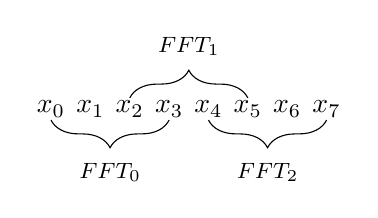
\begin{tikzpicture}
 		\tikzstyle{box} = [draw,inner sep=7,minimum size=57,line 
 		width=1, very thick, draw=black, fill=black!20, text width=100, text centered]
 		\tikzstyle{invisible} = [outer sep=0,inner sep=0,minimum size=0]
 		\tikzstyle{stealth} = [-stealth, very thick]
 		
 		\node [] at (-4,0) {$x_0$};
 		\node [] at (-3.5,0) {$x_1$};
 		\node [] at (-3,0) {$x_2$};
 		\node [] at (-2.5,0) {$x_3$};
 		\node [] at (-2,0) {$x_4$};
 		\node [] at (-1.5,0) {$x_5$};
 		\node [] at (-1,0) {$x_6$};
 		\node [] at (-0.5,0) {$x_7$};
 		
 		\draw [decorate,decoration={brace,amplitude=10pt,mirror,raise=4pt},yshift=0pt] (-4,0) -- (-2.5,0) node [black,midway,yshift=-0.8cm] {\footnotesize $FFT_0$};
 		\draw [decorate,decoration={brace,amplitude=10pt,mirror,raise=4pt},yshift=0pt] (-1.5,0) -- (-3,0) node [black,midway,yshift=0.8cm] {\footnotesize $FFT_1$};
 		\draw [decorate,decoration={brace,amplitude=10pt,mirror,raise=4pt},yshift=0pt] (-2,0) -- (-0.5,0) node [black,midway,yshift=-0.8cm] {\footnotesize $FFT_2$};
 		\end{tikzpicture}
 	\end{center}
 	\item $mod(n)$ El módulo de cada una de las componentes de la señal $FFT(n)$, i.e., 513\footnote{Al modelo entran 250 componentes para reducir la carga computacional dado que reducir el espectro hasta los 3000Hz no hace perder mucha calidad del sonido.}.
 	\item $\widetilde{mod}(n)$ El módulo de cada una de las componentes de la señal $FFT(n)$ con el ruido eliminado por la red neuronal.
 	\item $fase(n)$ La fase de cada una de las componentes de la señal $FFT(n)$, i.e., 513 componentes.
 	\item $imag(n)$ El vector con las componentes de la \gls{FFT} sin el ruido, para ello se reconstruye el número complejo a partir del módulo y la fase $imag(n)_i = \widetilde{mod}(n)_i\cdot e^{j\cdot fase(n)_i}$.
 	\item $x_{out}(n)$ Las muestras de salida a $11025\frac{muestras}{segundo}$ tras pasar por la transformada inversa
 	\item $x_{out}(t)$ Las muestras analógicas listas para ser reproducidas por los altavoces, de nuevo esta salida la genera la tarjeta de sonido del equipo.
\end{itemize}

\subsection{Generación de datos de entrenamiento y validación}
Para el entrenamiento más rápido del modelo, se pueden pre-procesar todos los datos con la cadena de \gls{DSP} mostrada en la figura \ref{fig: model_chain} previo a la entrada a la red. Para ello, se ha utilizado el código mostrado en \ref{lst: data_converter}.

Este algoritmo consiste en solicitar la combinación de pistas de audio-ruido a la base de datos para los ruidos solicitados. El algoritmo va a ser entrenado únicamente para un tipo de ruido debido a la cantidad de datos y al tiempo de entrenamiento que necesita para cada época. En este caso, se va a usar un ruido de la ciudad de Nueva York y se va a mezclar con todos los audiolibros. A esos audios se les va a calcular la transformada de Fourier a partir de la librería de \textit{señal de Scipy}. Para ello se va a utilizar la \gls{STFT} que genera una matriz de números complejos con todas las \glspl{FFT}. La salida se va a separar en módulo y fase y el módulo va a ser transformado de amplitud a decibelios. Este proceso se hace para tener valores más representativos. Los módulos de las mezclas de audios serán las entradas y los módulos de los audiolibros solos las salidas esperadas, todo en decibelios.

Finalmente, estos datos junto con sus metadatos de generación serán almacenados en un formato binario de acceso indexado muy ampliamente usado por la comunidad para el procesado de datos a grandes escalas en local, el \gls{HDF5}.

\section{Modelo de capas \acrshort{LSTM}}
Este trabajo presenta como solución al problema un modelo de capas \gls{LSTM}. Previo al diseño del propio modelo, cabe destacar los tipos de arquitecturas que se pueden usar en las redes recurrentes, es decir, cuando se trabaja con secuencias.
\subsection{Tipos de arquitectura}
Cuando se trabaja con redes neuronales recurrentes existen diferentes tipos de arquitecturas en función del número de elementos del eje tiempo que se introduzcan en la red, en el caso de este trabajo sería cuantos vectores \gls{FFT} tiene el algoritmo en cuenta, dado que un instante de tiempo viene representado por un vector \gls{FFT} completo.

\begin{figure}[ht!]
	\centering
	\resizebox{\textwidth}{!}{
		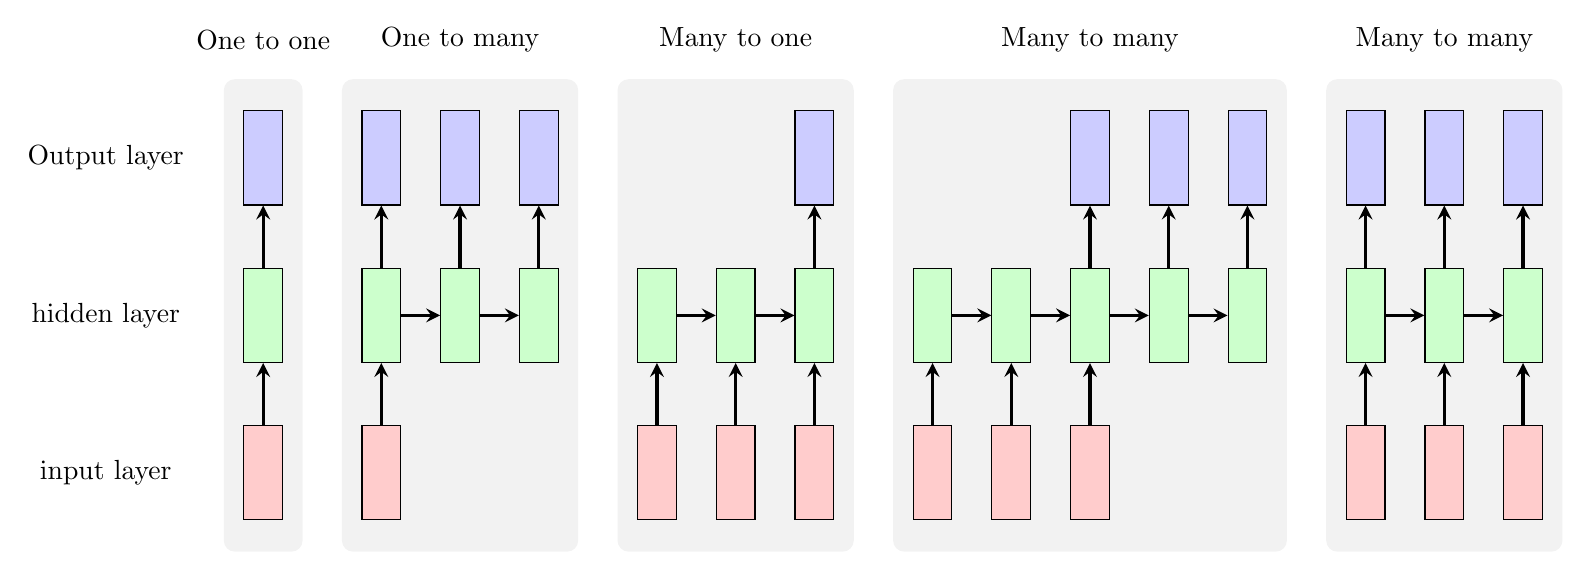
\begin{tikzpicture}
		\tikzstyle{input} = [draw,inner sep=7,minimum size=10, draw=black, fill=red!20, text width=20, text centered,rotate=90]
		\tikzstyle{hidden} = [draw,inner sep=7,minimum size=10, draw=black, fill=green!20, text width=20, text centered,rotate=90]
		\tikzstyle{output} = [draw,inner sep=7,minimum size=10, draw=black, fill=blue!20, text width=20, text centered,rotate=90]
		\tikzstyle{invisible} = [outer sep=0,inner sep=0,minimum size=0]
		\tikzstyle{stealth} = [-stealth, very thick]
		\fill [rounded corners, fill=gray!10] (-4,3.5) rectangle (-3,-2.5);
		\fill [rounded corners, fill=gray!10] (-2.5,3.5) rectangle (0.5,-2.5);
		\fill [rounded corners, fill=gray!10] (1,3.5) rectangle (4,-2.5);
		\fill [rounded corners, fill=gray!10] (4.5,3.5) rectangle (9.5,-2.5);
		\fill [rounded corners, fill=gray!10] (10,3.5) rectangle (13,-2.5);
		\node [input] (v1) at (-3.5,-1.5) {};
		\node [hidden] (v2) at (-3.5,0.5) {};
		\node [output] (v3) at (-3.5,2.5) {};
		\node [input] (v4) at (-2,-1.5) {};
		\node [hidden] (v5) at (-2,0.5) {};
		\node [hidden] (v7) at (-1,0.5) {};
		\node [hidden] (v8) at (0,0.5) {};
		\node [output] (v6) at (-2,2.5) {};
		\node [output] (v9) at (-1,2.5) {};
		\node [output] (v10) at (0,2.5) {};
		\node [input] (v11) at (1.5,-1.5) {};
		\node [input] (v13) at (2.5,-1.5) {};
		\node [input] (v15) at (3.5,-1.5) {};
		\node [hidden] (v12) at (1.5,0.5) {};
		\node [hidden] (v14) at (2.5,0.5) {};
		\node [hidden] (v16) at (3.5,0.5) {};
		\node [output] (v17) at (3.5,2.5) {};
		\node [input] (v18) at (5,-1.5) {};
		\node [input] (v20) at (6,-1.5) {};
		\node [input] (v22) at (7,-1.5) {};
		\node [hidden] (v19) at (5,0.5) {};
		\node [hidden] (v21) at (6,0.5) {};
		\node [hidden] (v23) at (7,0.5) {};
		\node [hidden] (v25) at (8,0.5) {};
		\node [hidden] (v27) at (9,0.5) {};
		\node [output] (v24) at (7,2.5) {};
		\node [output] (v26) at (8,2.5) {};
		\node [output] (v28) at (9,2.5) {};
		\node [input] (v29) at (10.5,-1.5) {};
		\node [input] (v32) at (11.5,-1.5) {};
		\node [input] (v35) at (12.5,-1.5) {};
		\node [hidden] (v30) at (10.5,0.5) {};
		\node [hidden] (v33) at (11.5,0.5) {};
		\node [hidden] (v36) at (12.5,0.5) {};
		\node [output] (v31) at (10.5,2.5) {};
		\node [output] (v34) at (11.5,2.5) {};
		\node [output] (v37) at (12.5,2.5) {};
		\draw [stealth] (v1) edge (v2);
		\draw [stealth] (v2) edge (v3);
		\draw [stealth] (v4) edge (v5);
		\draw [stealth] (v5) edge (v6);
		\draw [stealth] (v5) edge (v7);
		\draw [stealth] (v7) edge (v8);
		\draw [stealth] (v7) edge (v9);
		\draw [stealth] (v8) edge (v10);
		\draw [stealth] (v11) edge (v12);
		\draw [stealth] (v13) edge (v14);
		\draw [stealth] (v15) edge (v16);
		\draw [stealth] (v12) edge (v14);
		\draw [stealth] (v14) edge (v16);
		\draw [stealth] (v16) edge (v17);
		\draw [stealth] (v18) edge (v19);
		\draw [stealth] (v20) edge (v21);
		\draw [stealth] (v22) edge (v23);
		\draw [stealth] (v23) edge (v24);
		\draw [stealth] (v25) edge (v26);
		\draw [stealth] (v27) edge (v28);
		\draw [stealth] (v19) edge (v21);
		\draw [stealth] (v21) edge (v23);
		\draw [stealth] (v23) edge (v25);
		\draw [stealth] (v25) edge (v27);
		\draw [stealth] (v29) edge (v30);
		\draw [stealth] (v30) edge (v31);
		\draw [stealth] (v32) edge (v33);
		\draw [stealth] (v33) edge (v34);
		\draw [stealth] (v35) edge (v36);
		\draw [stealth] (v36) edge (v37);
		\draw [stealth] (v30) edge (v33);
		\draw [stealth] (v33) edge (v36);
		
		\node [invisible] at (-3.5,4) {One to one};
		\node [invisible] at (-1,4) {One to many};
		\node [invisible] at (2.5,4) {Many to one};
		\node [invisible] at (7,4) {Many to many};
		\node [invisible] at (11.5,4) {Many to many};
		\node [invisible] at (-5.5,-1.5) {input layer};
		\node [invisible] at (-5.5,0.5) {hidden layer};
		\node [invisible] at (-5.5,2.5) {Output layer};
		\end{tikzpicture}
	}      
	\caption{Arquitecturas de modelo}%\cite{karpathy}.
	\label{fig: model_archs}
\end{figure}

En la figura \ref{fig: model_archs} se pueden ver las diferentes arquitecturas que se pueden utilizar cuando se realiza un modelo\cite{karpathy}. En cada tipo de arquitectura, la capa roja representa la capa de entrada, para cada capa de entrada, la entrenada es un vector. La capa verde representa las capas ocultas con sus respectivas propagaciones de estado y las azules, las salidas. Se ha respetado la nomenclatura en inglés original de la bibliografía.

Un ejemplo de cada tipo sería:
\begin{itemize}
	\item \textbf{One to one}\arrowTikz{0}clasificación de imágenes, una entrada (matriz de la imagen), una salida, la categoría.
	\item \textbf{One to many}\arrowTikz{0}generación de títulos para imágenes, una entrada (matriz de la imagen), varias salidas, las diferentes palabras.
	\item \textbf{Many to one}\arrowTikz{0}análisis de sentimiento, entran varias palabras, se clasifica como positiva o negativa.
	\item \textbf{Many to many}\arrowTikz{0}traducción de texto, varias palabras en un idioma a la entrada y varias a la salida en otro idioma.
	\item \textbf{Many to many}\arrowTikz{0}entradas y salidas sincronizadas, clasificación de vídeo.
\end{itemize}
\subsection{Arquitectura del modelo}
Como se explicó anteriormente, las frecuencias fundamentales de la voz y sus armónicos son continuos en el tiempo, de ahí que estudiar cada \gls{FFT} como un evento independiente sería menos efectivo por tanto, la arquitectura en la cual la entrada es un instante de tiempo no tiene sentido porque se analizaría cada \gls{FFT} como un evento independiente. Como lo que se espera es una única \gls{FFT} de salida, la arquitecturas que se probaron durante el trabajo fueron y \textbf{one to one} \textbf{many to one}. Aquí cabe destacar que hay dos grandes posibilidades para el caso \textbf{many to one}:
\begin{itemize}
	\item Entrada de varias \glspl{FFT} anteriores a la actual y limpias de ruido (es decir darle varias salidas anteriores como entrada) y la \gls{FFT} con ruido actual
	\item Entrada de varias \glspl{FFT} anteriores a la actual y la actual pero todas con ruido.
\end{itemize}
Este trabajo se va a implementar la segunda de las opciones porque en la primera, se realimenta la salida, algo que con el estado de la celda ya tiene información de ello y, tiene el problema añadido que, mientras la red no funcione, las \glspl{FFT} ''limpias'' de ruido realmente no lo están.

La entrada al algoritmo será, por tanto, una serie de \glspl{FFT} de 1024 puntos calculadas a una señal de $11025\frac{muestras}{segundo}$ lo que implica que la frecuencia de muestreo de las \glspl{FFT} es 0.0464, es decir, unas 20 \glspl{FFT} por segundo, dado que el overlap es del 50\%. El rango de espectro es de 0 a 5512 hercios, una frecuencia muy alta para la voz humana, por esta razón se van a recortar las \glspl{FFT} a la entrada hasta los 3000 hercios, lo que reduce la matriz de entrada a casi la mitad. De este modo, el tamaño de la \gls{FFT} a la entrada es de 250 componentes.

El modelo consiste en tres capas \gls{LSTM} de 512 celdas y una capa de neuronas totalmente conectadas \textit{Dense} con 250 neuronas, dado el tamaño de la \gls{FFT}. Esto genera una red de $\approx6M$ parámetros. En \ref{lst: model_resume} se puede ver el resumen de la red y la interconexión de las capas. Cabe destacar que las \gls{LSTM} requieren de un tensor de tres dimensiones donde la primera es el número de elementos (típicamente tamaño del batch), la segunda, el número de pasos temporales y, la tercera, el número de parámetros, en este caso, las 250 bandas de frecuencia.

\begin{lstlisting}[basicstyle=\tiny\ttfamily, caption={Resumen del modelo},captionpos=b, label={lst: model_resume},frame=tb,
xleftmargin=.2\textwidth, xrightmargin=.2\textwidth]
_________________________________________________________________
Layer (type)                 Output Shape              Param #   
=================================================================
lstm (LSTM)                  (None, 1, 512)            1562624   
_________________________________________________________________
lstm_1 (LSTM)                (None, 1, 512)            2099200   
_________________________________________________________________
lstm_2 (LSTM)                (None, 512)               2099200   
_________________________________________________________________
dense (Dense)                (None, 250)               128250    
=================================================================
Total params: 5,889,274
Trainable params: 5,889,274
Non-trainable params: 0
_________________________________________________________________
\end{lstlisting}

\subsubsection{Generador de secuencias}
Para poder entrenar el modelo con una gran cantidad de datos que no quepan en la memoria \gls{RAM} del ordenador de entrenamiento, se requiere de un generador de secuencias. Este algoritmo se va a encargar de preparar los datos en bloques del tamaño del batch para entrenar con ellos el modelo.

En este caso, los datos han sido pre-procesados previamente y almacenados en el formato \gls{HDF5}, como se explicó en el apartado anterior. Esto se ha hecho para reducir la carga computacional dado que la carga del audio y el ruido, la mezcla de ambos y el cálculo de la \gls{STFT} es un proceso costoso computacionalmente. De este modo, el \textit{Generador de Secuencias} sólo debe cargar los datos, normalizarlos y juntarlos en grupos del tamaño de pasos temporales y el tamaño del batch. En \textcolor{red}{REFERENCIA} se tiene el código que implementa esta parte del proyecto. A continuación se detallan cada una de las partes.

\paragraph{Carga de datos}

La carga de datos consiste en extraer las \glspl{FFT} que se encuentran almacenadas en el \gls{HDD} y almacenarlas en \gls{RAM}. Este paso se divide en dos partes:
\begin{itemize}
	\item Parseo de la estructura del archivo para contabilizar el número de \gls{FFT} total\arrowTikz{0}ejecutado 1 vez.
	\item Carga de las correspondientes \glspl{FFT} y actualización de los correspondientes índices para generar un tensor del tamaño del batch\arrowTikz{0}ejecutado tantas veces como batches hay en el \gls{HDF5}.
\end{itemize}

El archivo generado para 1500 de los audios que tengan una tasa de muestreo múltiplo de la del modelo 11025 y para un único ruido tiene un tamaño de 294 GBytes. A modo explicativo se presenta en las figuras \ref{fig: hdf5_struct} y \ref{fig: hdf5_struct2} un ejemplo de la estructura del \gls{HDF5} y cómo se encuentran los datos.

\begin{figure}[h!]
	\centering
	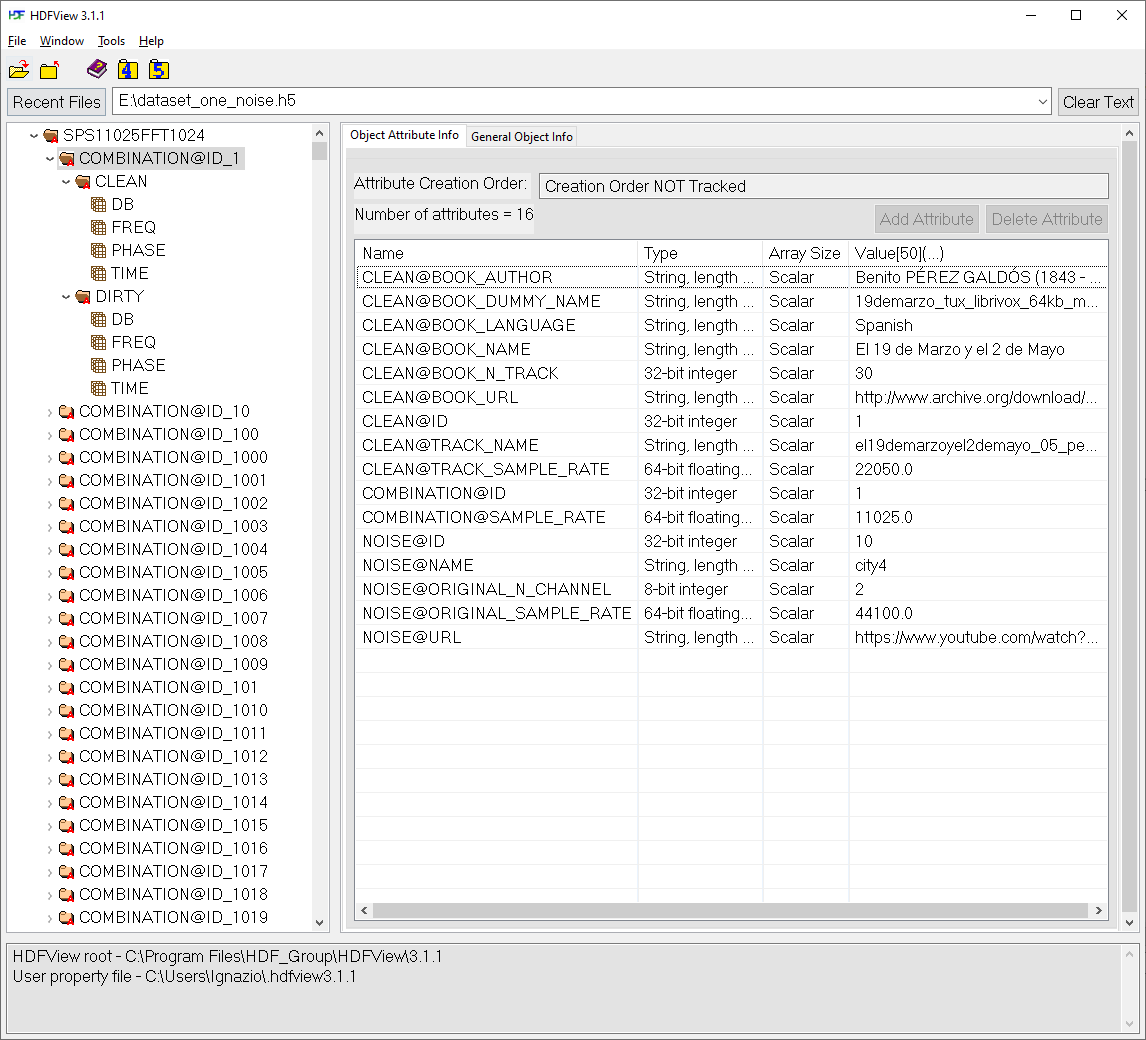
\includegraphics[width=0.9\columnwidth]{figures/HDF5_struct}
	\caption{Estructura del archivo \gls{HDF5}}
	\label{fig: hdf5_struct}
\end{figure}

\begin{figure}[h!]
	\centering
	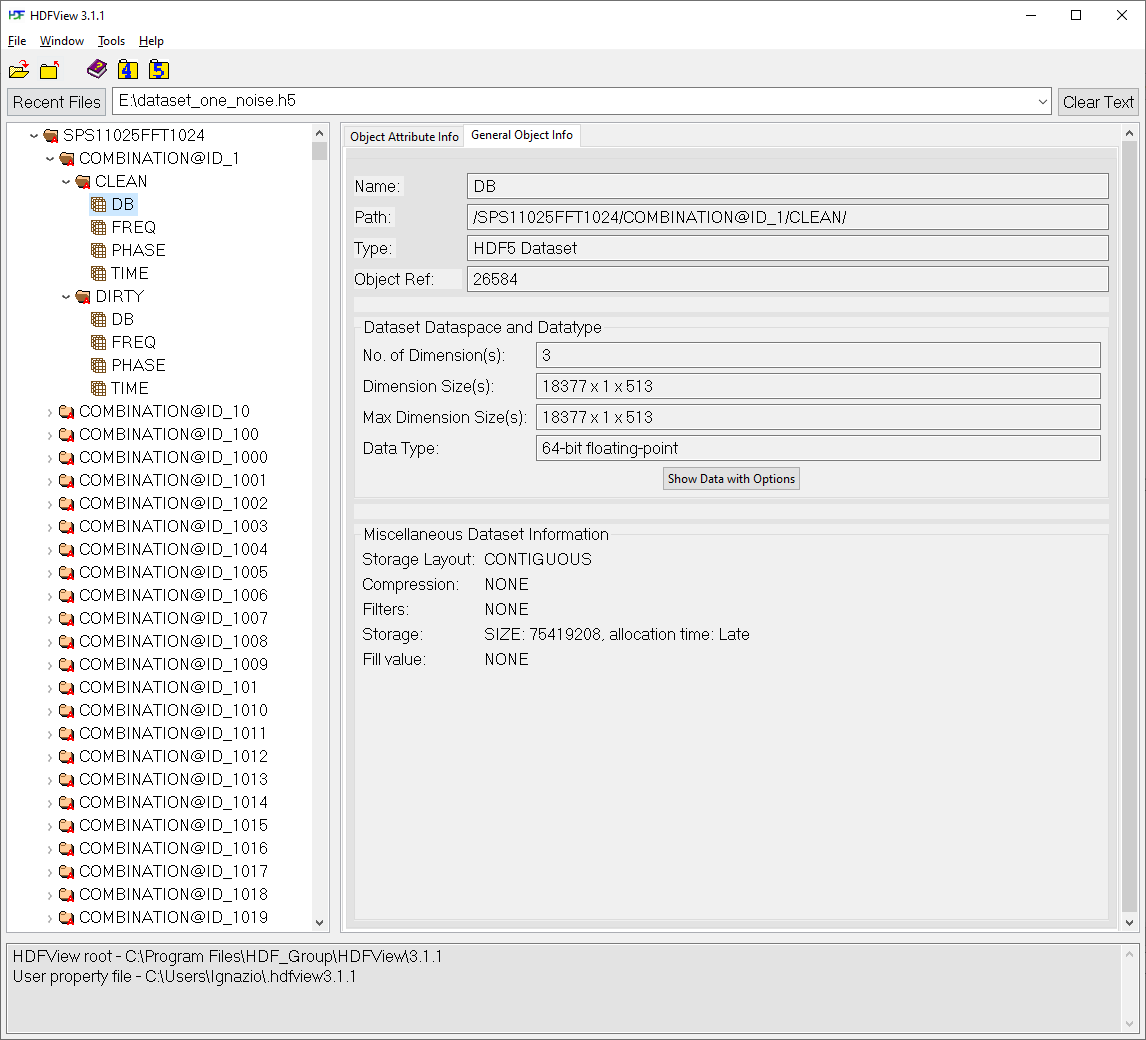
\includegraphics[width=0.9\columnwidth]{figures/HDF5_struct2}
	\caption{Estructura de los datos almacenados en el archivo \gls{HDF5}}
	\label{fig: hdf5_struct2}
\end{figure}

\paragraph{Normalización}

El proceso de normalización de los datos es una de las partes más importantes y puede ser el causante de que el modelo no funcione correctamente. En este caso, el apartado se refiere a la normalización de las potencias de las bandas frecuenciales calculadas en decibelios. Existe otra normalización que consiste en cargar los datos de los audios a una señal temporal normalizada, i.e., en el rango $\left[\text{-}1,1\right]$.

La normalización de las bandas se justifica como que cada banda es una señal y se normaliza aplicando la ecuación \ref{eq: norm} que representa la normalización de una componente genérica de potencia $i$ de una banda genérica $b$.

\begin{align}
\nonumber
P_{norm~b,i} &= \frac{P_{b,i} \text{-}\mu}{\sigma} \\ \nonumber
donde: \\ \nonumber
\mu&=\frac{\sum_{i=0}^{N}P_{b, i}}{N} \\ \nonumber
\sigma &= \sqrt{ \left( \frac{\sum_{i=0}^{N}{ {\left| P_{b, i} \text{-} \mu \right|}^2}}{N} \right) }
\end{align}
\equationset{Ecuación de la normalización.}\label{eq: norm}

\paragraph{Carga en grupos del tamaño del batch}